\documentclass[10pt]{article}
\usepackage[margin=0.7in,top=0.55in,bottom=0.55in]{geometry}
\usepackage{graphicx}
\usepackage{xcolor}
\usepackage{booktabs}
\usepackage{enumitem}
\usepackage{titlesec}
\usepackage[hidelinks]{hyperref}
\usepackage{array}
\usepackage{parskip}

\definecolor{accent}{HTML}{2A78D6}
\definecolor{warncol}{HTML}{EB6834}
\definecolor{inksoft}{HTML}{52514E}
\definecolor{muted}{HTML}{898781}
\definecolor{rule}{HTML}{E1E0D9}

\titleformat{\section}{\large\bfseries}{}{0pt}{}
\titlespacing*{\section}{0pt}{8pt}{3pt}
\titleformat{\subsection}{\normalsize\bfseries\color{inksoft}}{}{0pt}{}
\titlespacing*{\subsection}{0pt}{6pt}{2pt}

\setlength{\parindent}{0pt}
\setlength{\parskip}{3pt}
\pagestyle{empty}

\begin{document}

{\LARGE \bfseries AR1 Simulation Comparison}

\vspace{2pt}
{\color{inksoft} {\small\ttfamily n=500, m=1000, AR1 $\rho$=0.3, $\sigma_s$=0.3, 100 reps per F$_{ST}$}}

\vspace{3pt}
\noindent\rule{\linewidth}{0.4pt}

\section*{Main points}
\begin{itemize}[leftmargin=14pt, itemsep=1.5pt, topsep=1pt]
  \item R's free-intercept slope (\texttt{res\_reg\_free}) and Python's LDSC estimators (\texttt{h2\_ldsc\_nw}, \texttt{h2\_ldsc\_fixed\_nw}) are \textbf{different estimators}, not bugs: they differ in intercept constraint, LD-score source, and bias correction.
  \item \textbf{Bias correction explains most of the fixed-intercept gap} in the in-sample case. Python's default LD-score correction is a near-constant shift --- it barely moves the free-intercept slope (cancelled by centering) but closes most of the fixed-intercept mismatch at low-to-moderate F$_{ST}$.
  \item \textbf{A reference panel only works if it actually matches the sample's stratification.} With an independently-redrawn stratification vector $f$, the free-intercept estimator collapses toward zero on \emph{both} R and Python --- confirmed down to a correlation of $\approx$0 between the reference panel's LD score and the sample's $\chi^2$ statistic, even at F$_{ST}$=0 (no stratification at all) and even after scaling $n$ and $m$ up 4$\times$.
  \item \textbf{Sharing the same $f$ between the reference panel and the sample recovers the signal.} This isolates the mechanism precisely: a reference panel is only informative to the extent it matches the sample on the specific thing driving each SNP's LD-score magnitude. Once shared, both free- and fixed-intercept estimators recover a sensible shape in both languages.
  \item \textbf{Bias correction matters a lot for fixed intercept, in the reference-panel case too --- not just in-sample.} Removing R's bias correction from the reference-panel LD score (while Python keeps its own) blows the R-vs-Python gap out from $\pm$0.13 to as much as $-1.04$ at low F$_{ST}$. Free intercept is still essentially unaffected either way (differences under 0.01), exactly as the centering-cancels-a-constant-shift math predicts.
  \item A residual gap ($\sim$0.02--0.13, fixed intercept) remains even with bias correction matched on both sides --- pointing to something inside Python's IRWLS/jackknife regression machinery, not the LD score itself.
\end{itemize}

\section*{Section 1: In-sample LD scores}
Both R and Python recompute the LD score from each replicate's own data every time (no reference panel). R's columns are uncorrected; Python applies its default bias correction.

\begin{minipage}[t]{0.49\linewidth}
  \centering
  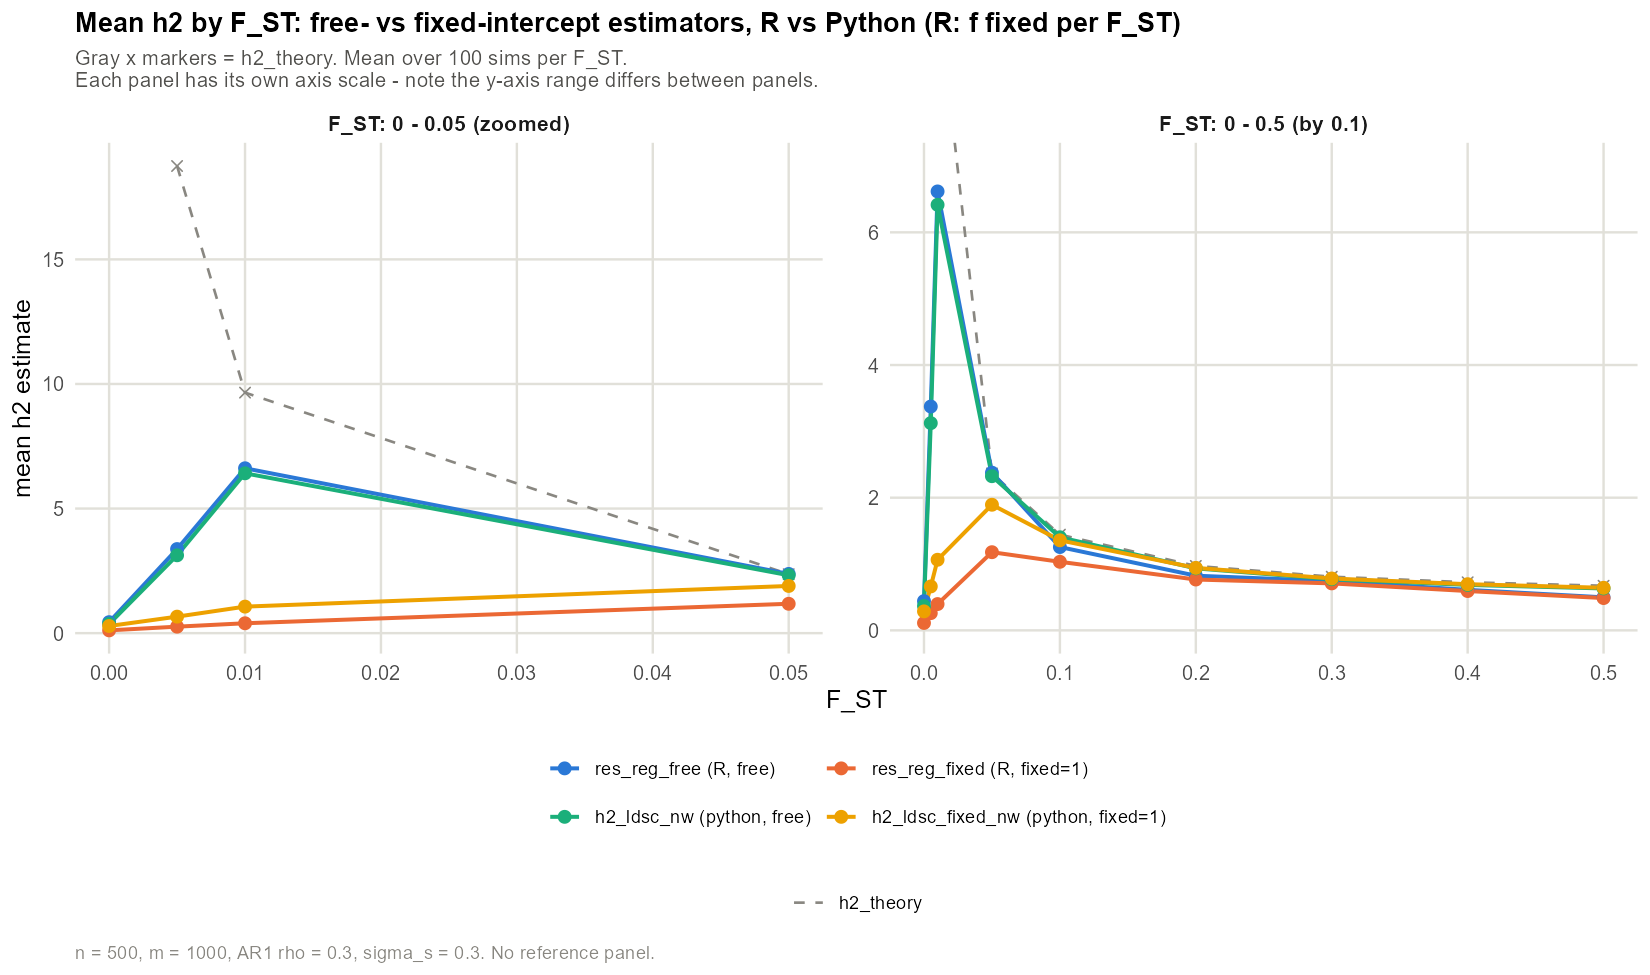
\includegraphics[width=\linewidth]{../figures/h2_by_fst_fixedf.png}\\[2pt]
  {\footnotesize\color{inksoft}\textbf{Figure 1.} Stratification vector $f$ fixed once per F$_{ST}$, shared across all 100 reps.}
\end{minipage}
\hfill
\begin{minipage}[t]{0.49\linewidth}
  \centering
  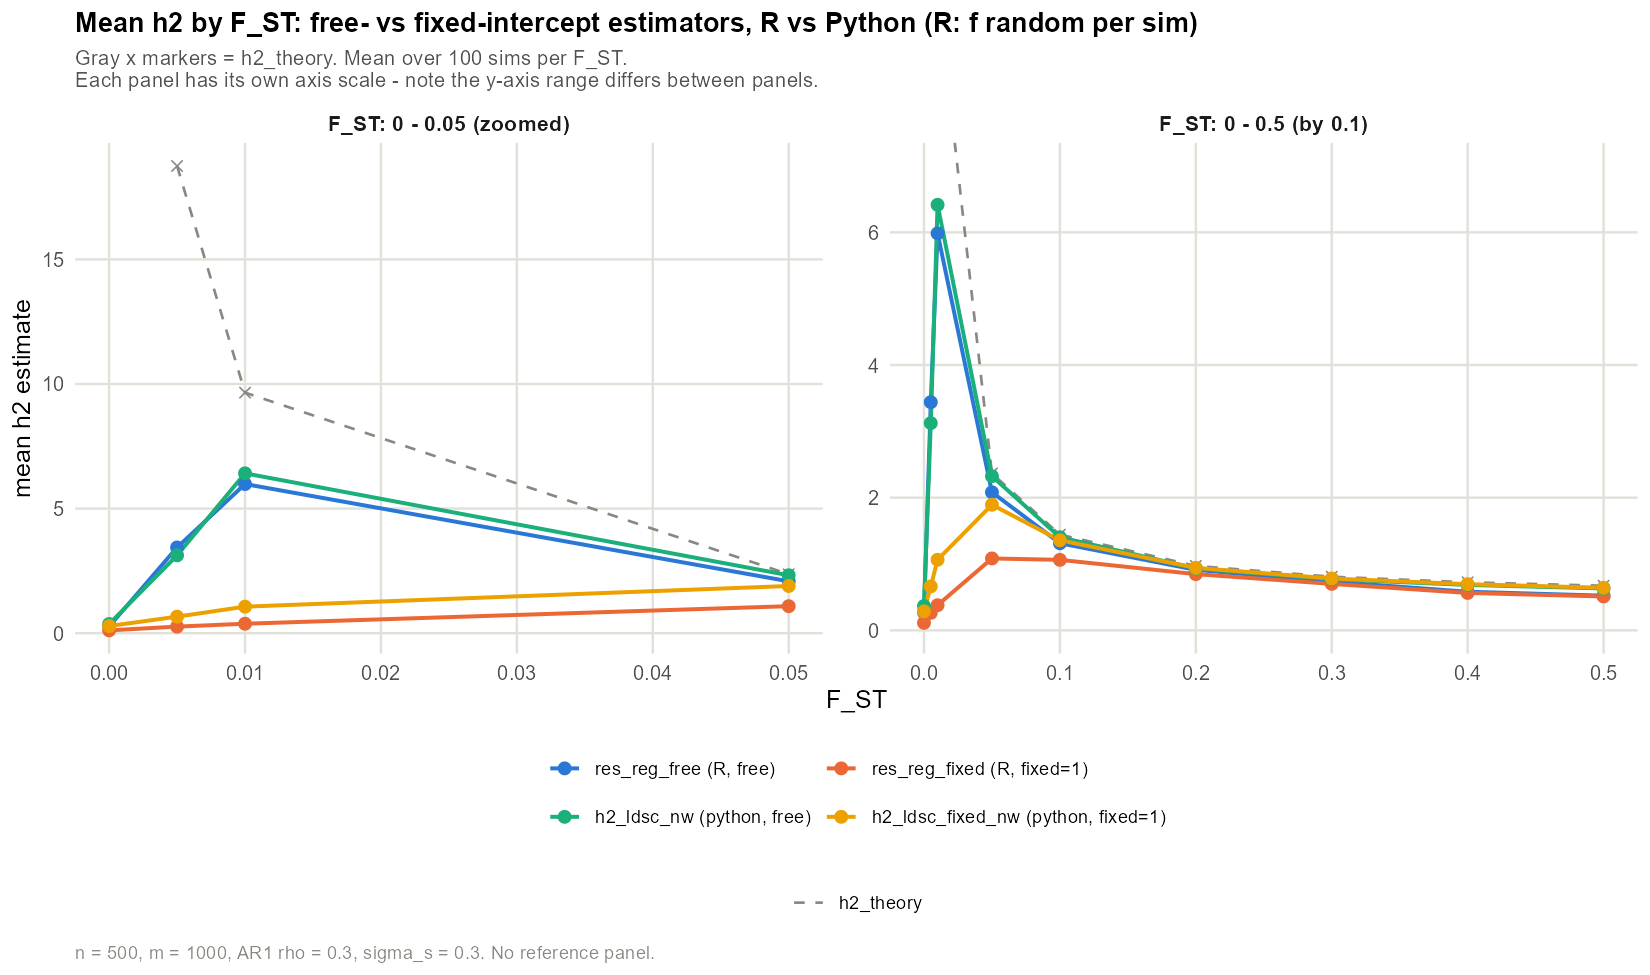
\includegraphics[width=\linewidth]{../figures/h2_by_fst_randf.png}\\[2pt]
  {\footnotesize\color{inksoft}\textbf{Figure 2.} Stratification vector $f$ redrawn fresh every replicate (matches Python's generative design; this is what makes $h2\_theory$ agree between R and Python).}
\end{minipage}

\section*{Section 2: Reference-panel LD scores, R's original (uncorrected) implementation}
Both sides use a separately-simulated reference panel (same generative process, independent individuals) for the LD score, reused across all 100 replicates. This is R's \emph{original} implementation, before bias correction was added to the R code --- R's reference-panel LD score has no correction term here, while Python's still applies its default bias correction. The only thing that changes between the two figures below is whether the reference panel's stratification draw $f$ is the \emph{same} one used to generate the 100 main replicates, or an independent one.

\begin{minipage}[t]{0.49\linewidth}
  \centering
  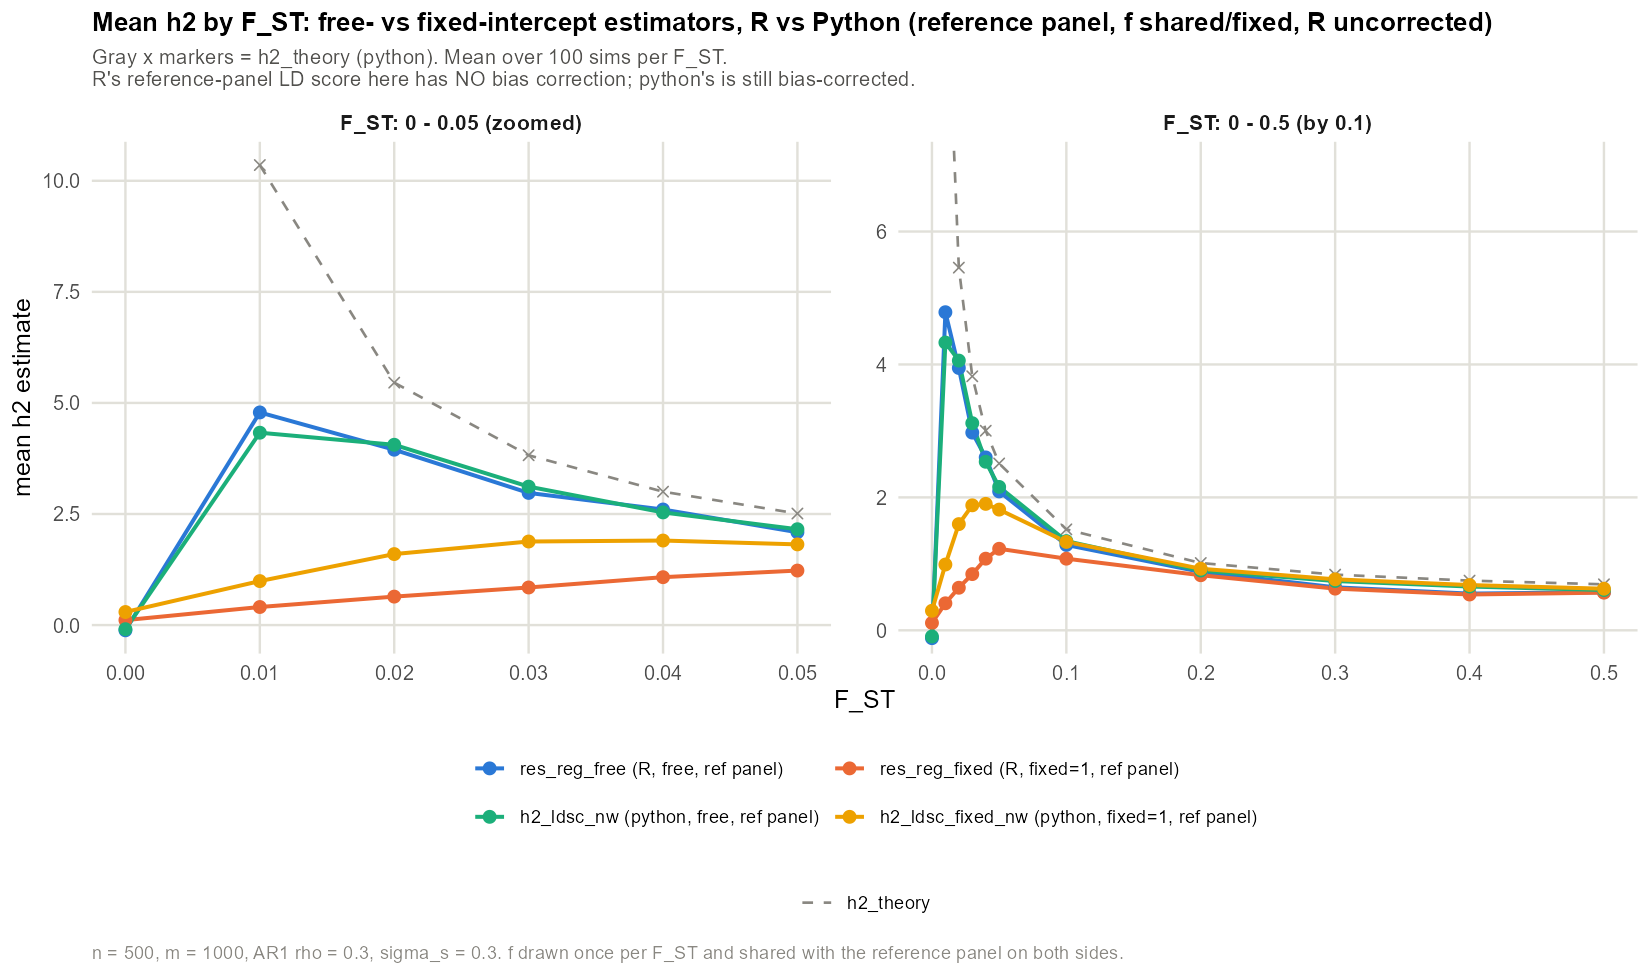
\includegraphics[width=\linewidth]{../figures/h2_by_fst_refpanel_fixedf_nobc.png}\\[2pt]
  {\footnotesize\color{inksoft}\textbf{Figure 3.} $f$ shared, R's reference LD score uncorrected. Free intercept recovers a sensible shape on both sides; fixed intercept has R sitting below Python.}
\end{minipage}
\hfill
\begin{minipage}[t]{0.49\linewidth}
  \centering
  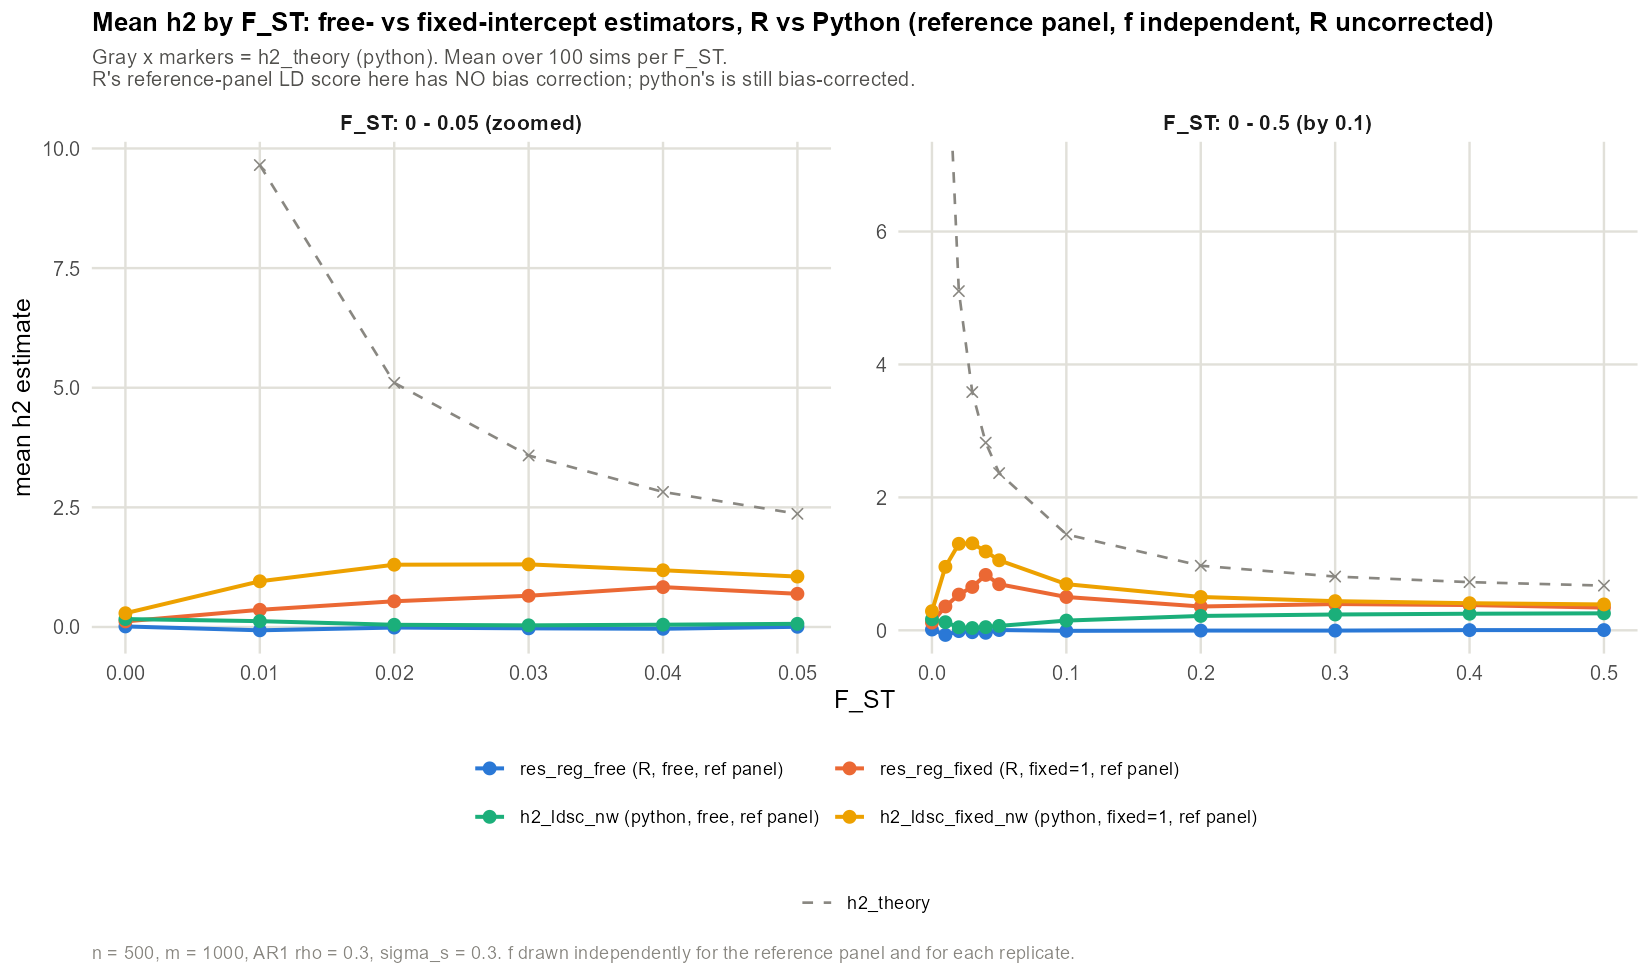
\includegraphics[width=\linewidth]{../figures/h2_by_fst_refpanel_indepf_nobc.png}\\[2pt]
  {\footnotesize\color{inksoft}\textbf{Figure 4.} $f$ independent, R's reference LD score uncorrected. Free intercept collapses toward zero on both R and Python; fixed intercept shows the widest R-vs-Python gap in the report.}
\end{minipage}

\section*{Section 3: Adding bias correction to R's reference-panel LD score}
Same two configurations as Section 2 (f shared / f independent), but now R's reference-panel LD score gets the same bias-correction term Python already applies. Fixed intercept moves substantially closer to Python; free intercept is essentially unchanged either way.

\begin{minipage}[t]{0.49\linewidth}
  \centering
  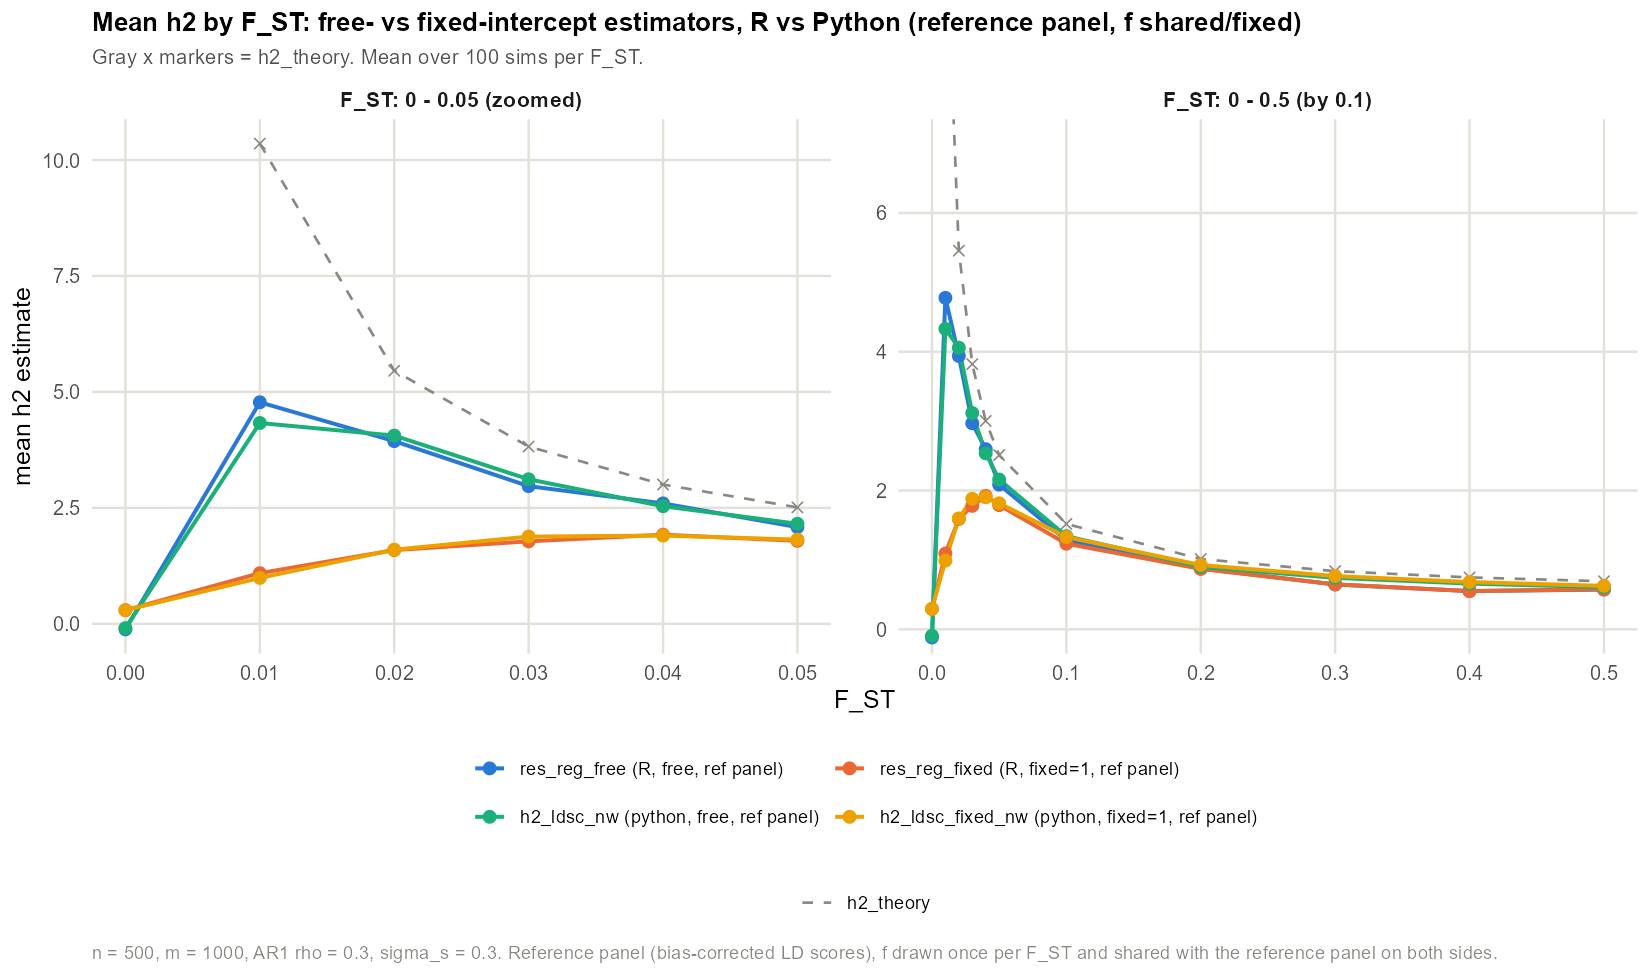
\includegraphics[width=\linewidth]{../figures/h2_by_fst_refpanel_fixedf.png}\\[2pt]
  {\footnotesize\color{inksoft}\textbf{Figure 5.} $f$ shared, R's reference LD score bias-corrected (matches Python's correction). Fixed intercept now tracks Python closely.}
\end{minipage}
\hfill
\begin{minipage}[t]{0.49\linewidth}
  \centering
  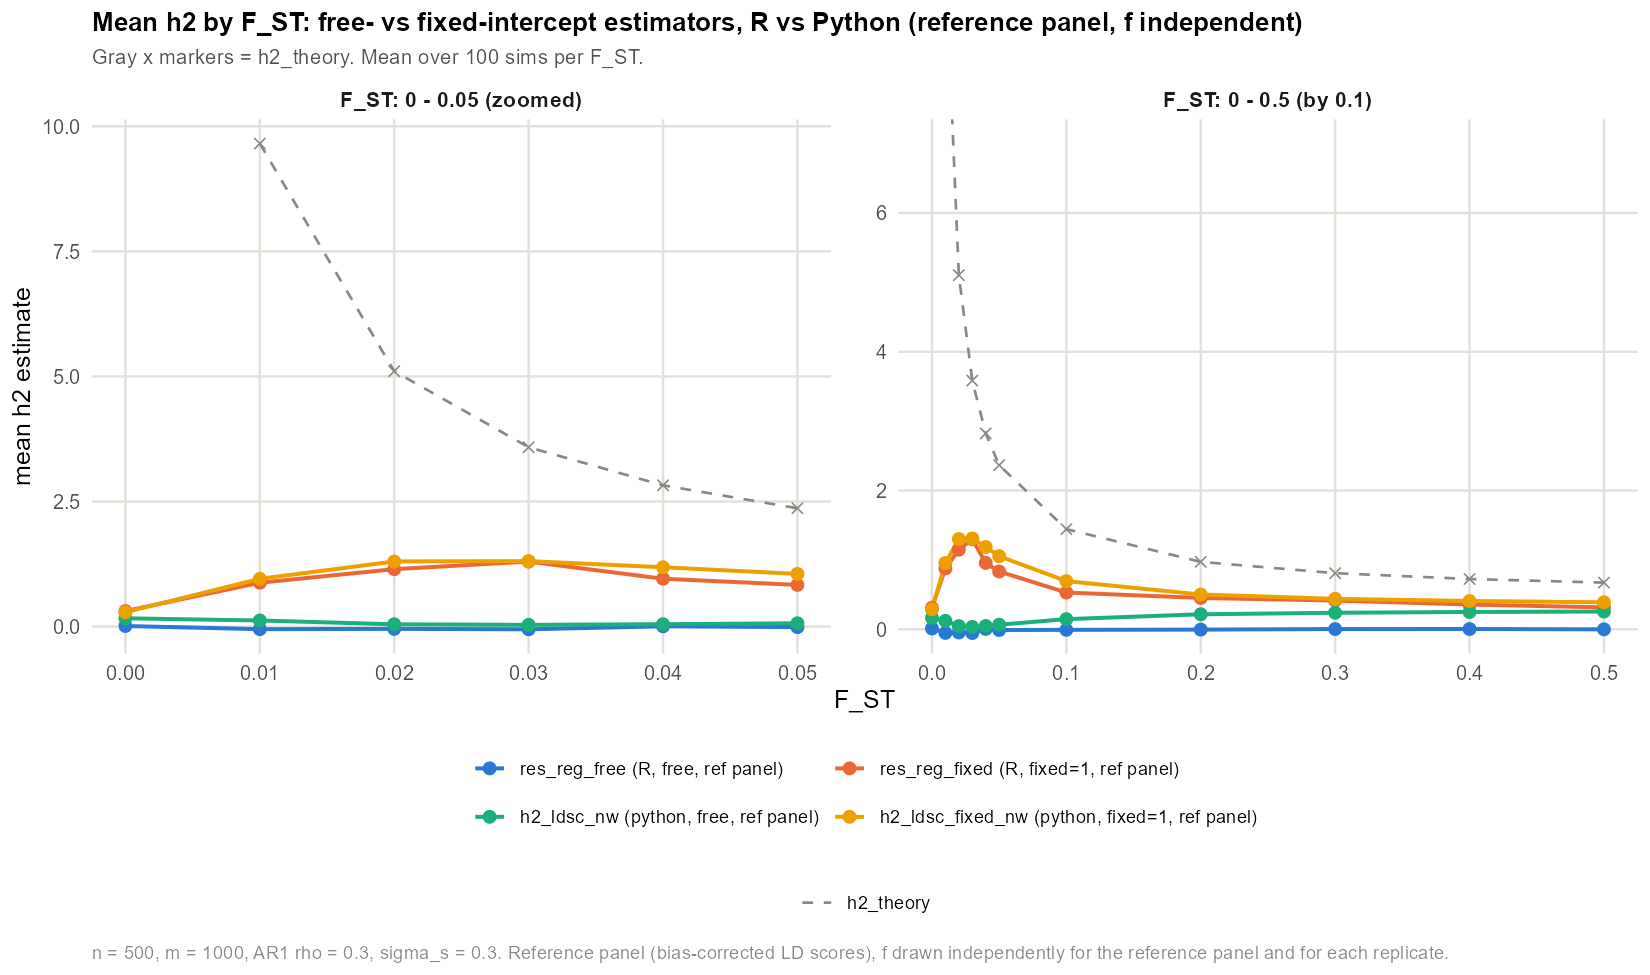
\includegraphics[width=\linewidth]{../figures/h2_by_fst_refpanel_indepf.png}\\[2pt]
  {\footnotesize\color{inksoft}\textbf{Figure 6.} $f$ independent, R's reference LD score bias-corrected. Free intercept still collapses toward zero on both sides --- bias correction doesn't touch that mechanism.}
\end{minipage}

\vspace{4pt}
\small
\renewcommand{\arraystretch}{1.15}
\noindent\begin{tabular}{r r r r r r}
\toprule
F$_{ST}$ & Python (fixed) & R, uncorrected (Fig.\ 3--4) & R, bias-corrected (Fig.\ 5--6) & diff (R$_{nobc}$ $-$ py) & diff (R$_{bc}$ $-$ py) \\
\midrule
0.00 & 0.294 & 0.111 & 0.295 & $-$0.183 & +0.001 \\
0.01 & 0.990 & 0.407 & 1.092 & $-$0.583 & +0.102 \\
0.02 & 1.598 & 0.641 & 1.590 & $-$0.958 & $-$0.008 \\
0.03 & 1.881 & 0.846 & 1.779 & $-$1.035 & $-$0.102 \\
0.04 & 1.903 & 1.078 & 1.922 & $-$0.825 & +0.019 \\
0.05 & 1.816 & 1.227 & 1.789 & $-$0.589 & $-$0.027 \\
0.10 & 1.330 & 1.078 & 1.234 & $-$0.252 & $-$0.096 \\
0.50 & 0.626 & 0.567 & 0.576 & $-$0.059 & $-$0.050 \\
\bottomrule
\end{tabular}
\normalsize

\section*{What drove each gap}
\small
\renewcommand{\arraystretch}{1.2}
\noindent\begin{tabular}{p{0.24\linewidth} p{0.37\linewidth} p{0.32\linewidth}}
\toprule
\textbf{Factor} & \textbf{Effect on free intercept} & \textbf{Effect on fixed intercept} \\
\midrule
Intercept constraint (free vs.\ fixed=1) & --- & Not the dominant cause once other factors are matched \\
Bias correction (near-constant LD-score shift), in-sample & None (cancelled by centering) & Closes most of the in-sample gap at low--mid F$_{ST}$ \\
Bias correction, reference panel (Figures 3--6) & None (diffs $<$0.01 regardless of $f$-sharing) & Large: removing it alone widens the R-vs-Python gap to $-$1.04 at low F$_{ST}$ \\
Reference panel with independent $f$ (Figures 4, 6) & Collapses toward noise (both languages) --- confirmed at F$_{ST}$=0 and up to 4$\times$ larger $n$,$m$ & Degraded but still informative \\
Reference panel with shared $f$ (Figures 3, 5) & Recovers a sensible shape in both languages & Recovers a sensible shape in both languages \\
Python's IRWLS/jackknife internals & Still unexplained & Best remaining candidate for the $\sim$0.02--0.13 residual \\
\bottomrule
\end{tabular}
\normalsize

{\footnotesize\color{muted} Open question: whether Python's \texttt{do\_ldsc\_regression} (weights=1, twostep=None path) is exactly mathematically identical to R's closed-form slope, or introduces a small systematic offset --- not yet traced through.}

\end{document}
